%!TEX root = ../TTK4550-MHT.tex
\section{Results}
\label{sec:results}

\subsection{Testing scheme}
The evaluation of the MHT algorithm is two-sided, firstly the algorithm must be able to track under challenging conditions, secondly it must be able to do this without having an ever growing computationally cost. The first performance metric is how well the algorithm is estimating the true position to the object it is tracking. This is measured as the Euclidean distance:
\begin{equation}
	\Delta P = \| \V{p}_{track}-\V{p}_{target} \|_2
\end{equation}
where the track is considered correct if $\Delta P \leq	\varepsilon_p$ for all t after initial convergence. If a track is deviating more that the threshold and is never within the threshold again, it is considered lost at the time-step it exceeded the threshold. If the track should converge after exceeding the threshold, it is considered restored at the time-step it is returning within the limit. The algorithm is tested on five scenarios:
\begin{itemize}
	\item Five fully cooperating ships
    \item Five partially cooperative ships
    \item Five ships avoiding obstacles with large space
    \item Five ships avoiding obstacles with little space
	\item Five parallel ships
\end{itemize}

\begin{figure}
    \centering   
    \begin{subfigure}{0.49\textwidth}
        \centering
        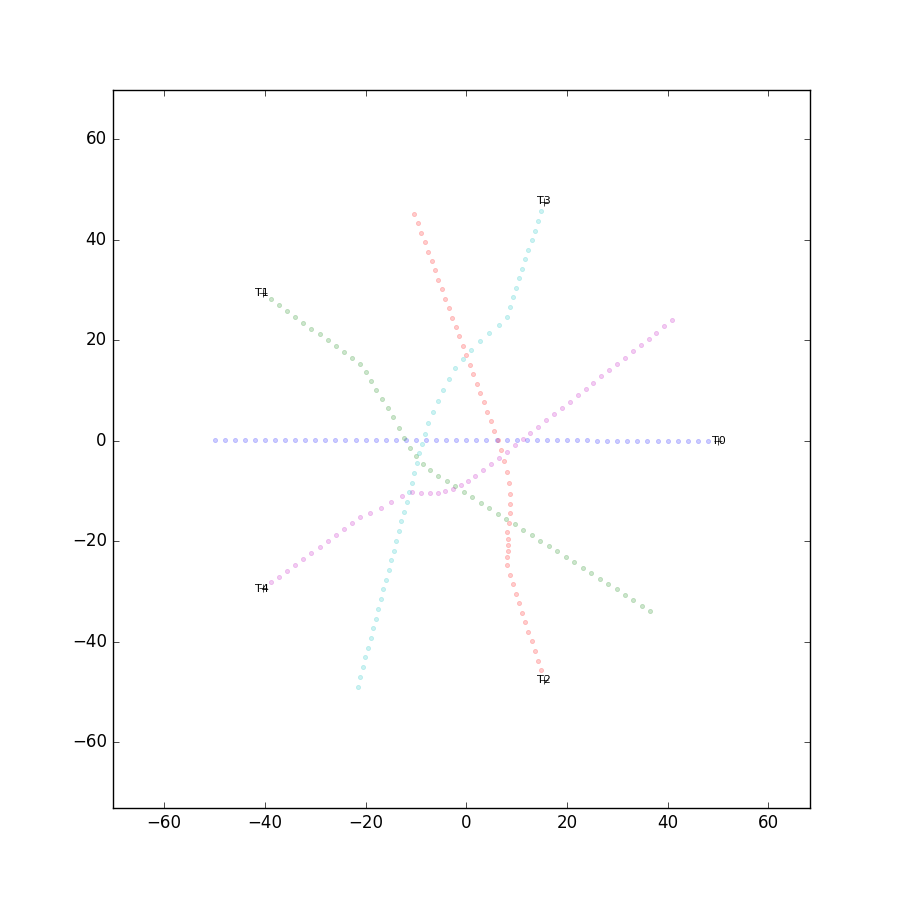
\includegraphics[clip, trim=2cm 1.5cm 2cm 2cm, height=0.3\textheight]{scenario1}
        \caption{First scenario}
    \end{subfigure}
    \begin{subfigure}{0.49\textwidth}
        \centering
        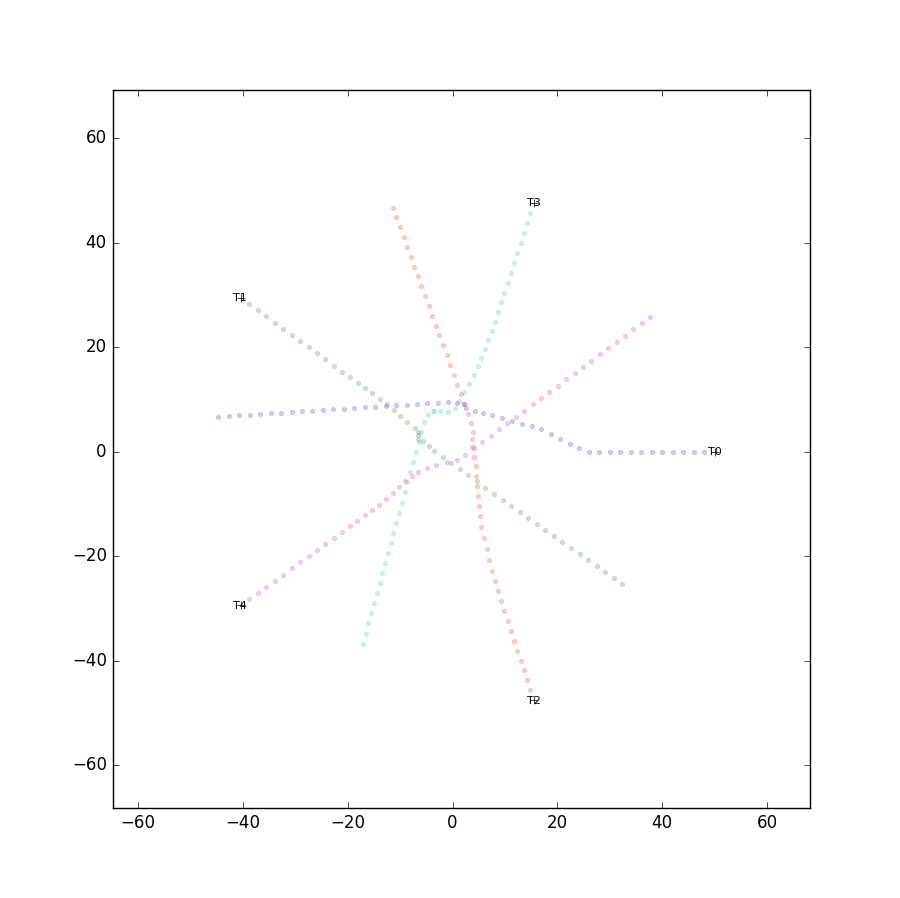
\includegraphics[clip, trim=2cm 1.5cm 2cm 2cm,height=0.3\textheight]{scenario2}
        \caption{Second scenario}
    \end{subfigure}
    \begin{subfigure}{0.49\textwidth}
        \centering
        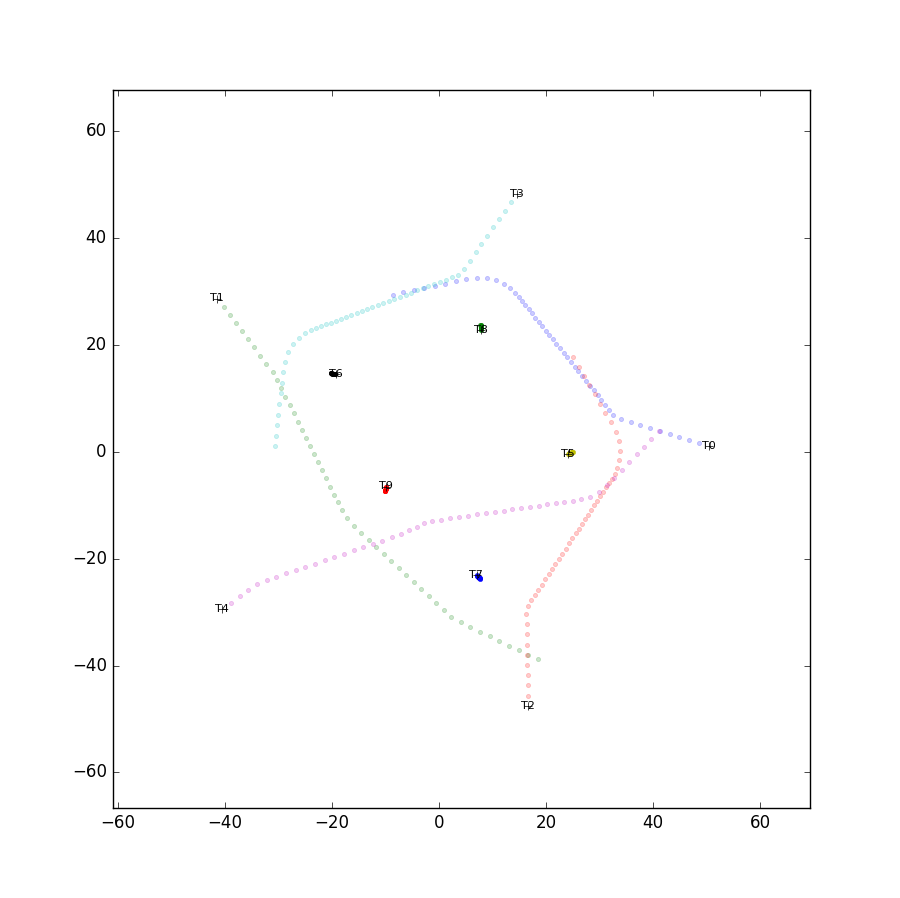
\includegraphics[clip, trim=2cm 1.5cm 2cm 2cm,height=0.3\textheight]{scenario3}
        \caption{Third scenario}
    \end{subfigure}
    \begin{subfigure}{0.49\textwidth}
        \centering
        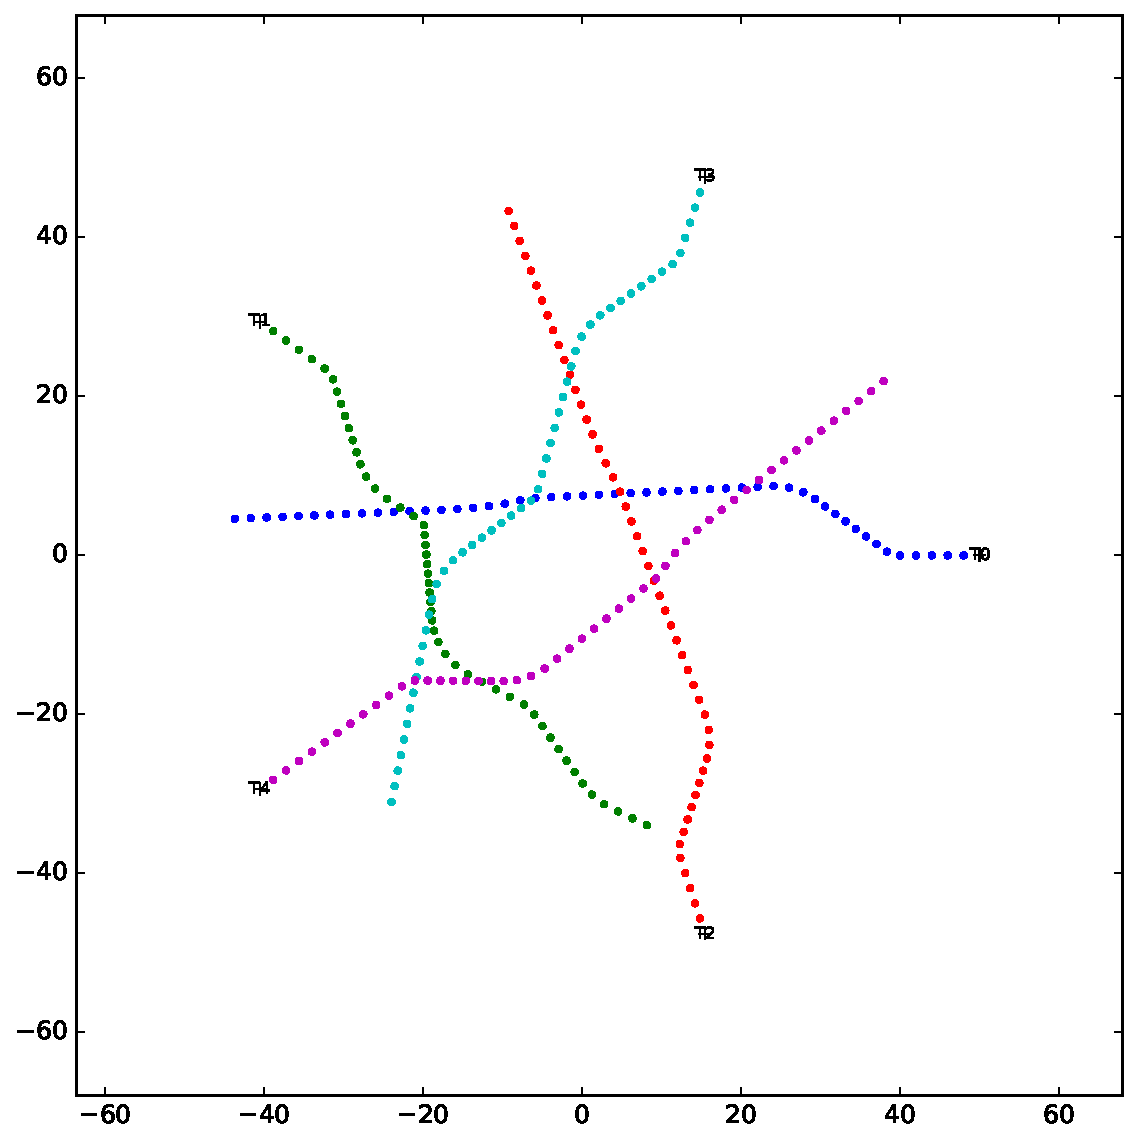
\includegraphics[clip, trim=2cm 1.5cm 2cm 2cm,height=0.3\textheight]{scenario4}
        \caption{Fourth scenario}
    \end{subfigure}
    \begin{subfigure}{0.49\textwidth}
        \centering
        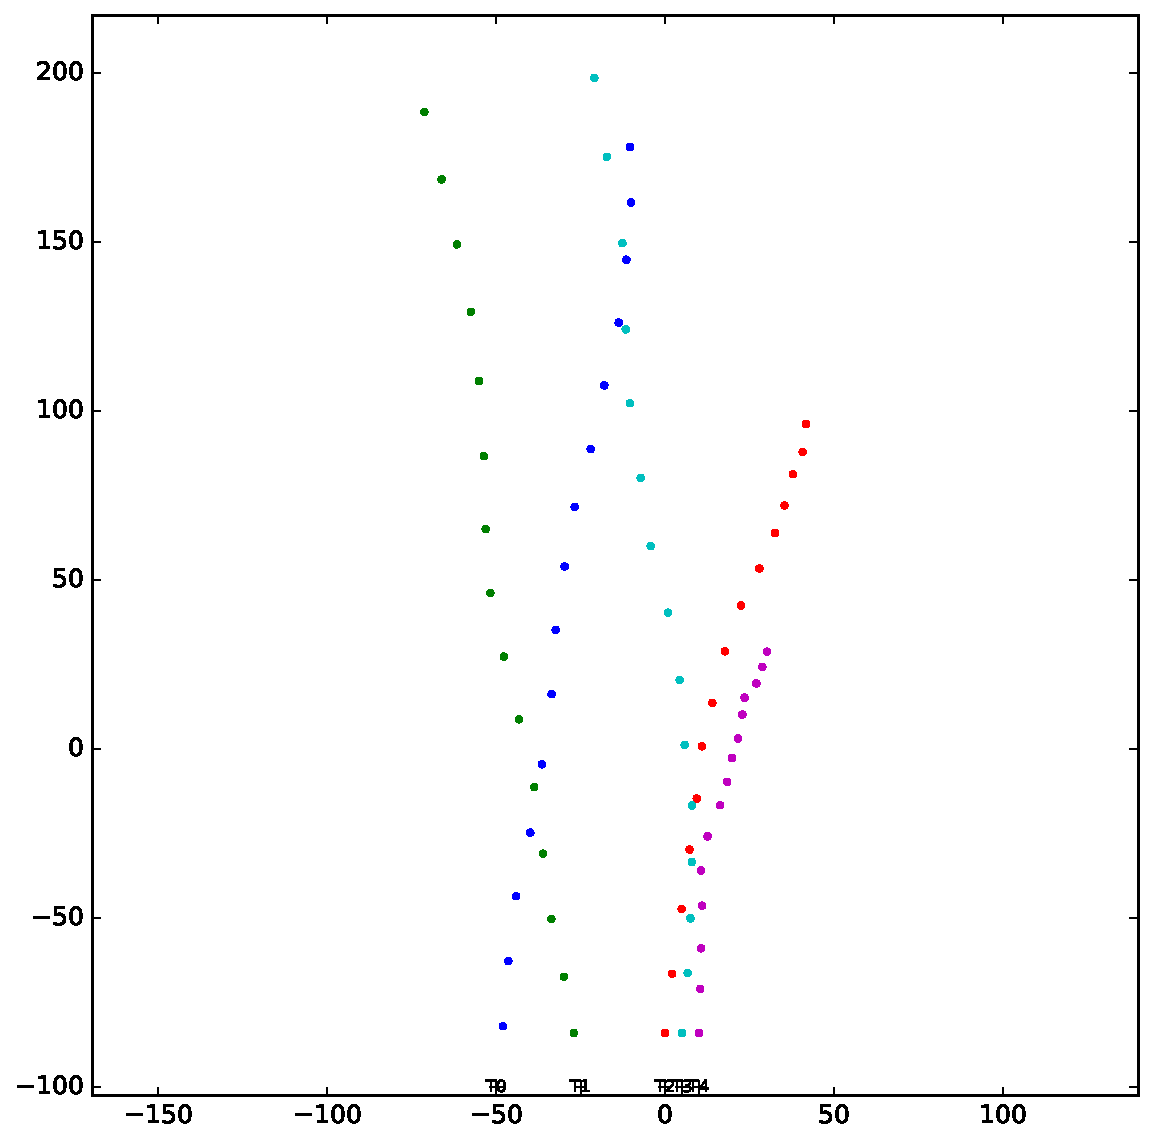
\includegraphics[height=0.29\textheight]{scenario5}
        \caption{Fifth scenario}
    \end{subfigure}
\end{figure}

\subsection{Simulation data}
Scenario one through four is generated as a recording of time and position from an Autonomous Surface Vessel (ASV)-simulator with collision avoidance (COLAV) which is a project under work by D. Kwame Minde Kufolaor at NTNU. The targets are configured such that they need to maneuver to avoid collision with each other, which allows for tracking of maneuvering targets in close proximity to each other. The fifth scenario is generated as a part of this project and is composed by linear parallel paths with hight measurement noise and system uncertainty.
%The third data-set is generated from Thomas Stenersen ASV simulator which was a part of this masters thesis. This simulator have several different pre-configured scenarios, and can also be modified to create any desired scenario.

\subsection{Simulations}
Scenario one through four was simulated with the following variations with all four solvers.
\begin{equation*}
\begin{split}
\V{P_D} &= \begin{bmatrix} 0.5 & 0.7 & 0.9 \end{bmatrix} \\
\V{N} &=\begin{bmatrix} 1 & 3 & 6 \end{bmatrix} \\
\V{\lambda_\phi} &=\begin{bmatrix} 0 & 1\cdot10^{-4} & 2\cdot10^{-4} & 4\cdot10^{-4} \end{bmatrix}
\end{split}
\end{equation*}
Each variant was simulated 100 times with different seeded random clutter measurements and miss detections. For each simulation, the estimated tracks was compared with the true tacks and categorised in successful and lost tracks. Figure \ref{fig:dynamic_agents_full_cooperation_cropped} to \ref{fig:dynamic_and_static_agents_narrow_space_cropped} show the averaged track loss percentage.

\subsection{Tracking performance}
\begin{figure}[H]
    \centering
    \textbf{Scenario 1}\par \medskip
    \begin{subfigure}{0.49\textwidth}
        \centering
        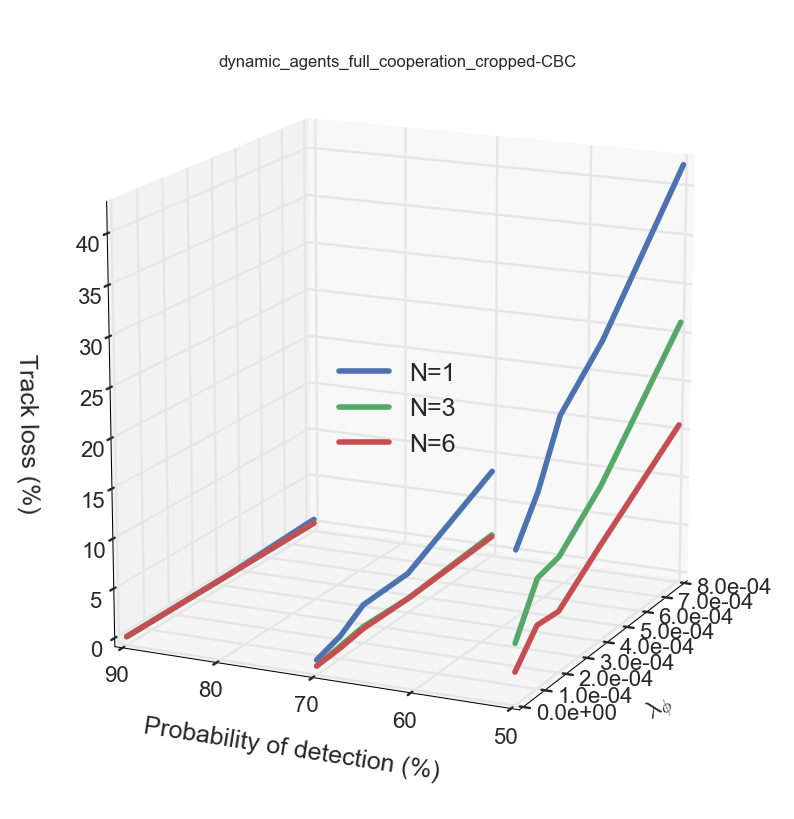
\includegraphics[clip, trim=0cm 0cm 0cm 2cm, width=\textwidth]{dynamic_agents_full_cooperation_cropped-CBC}
        \caption{CBC solver}
    \end{subfigure}
    \begin{subfigure}{0.49\textwidth}
        \centering
        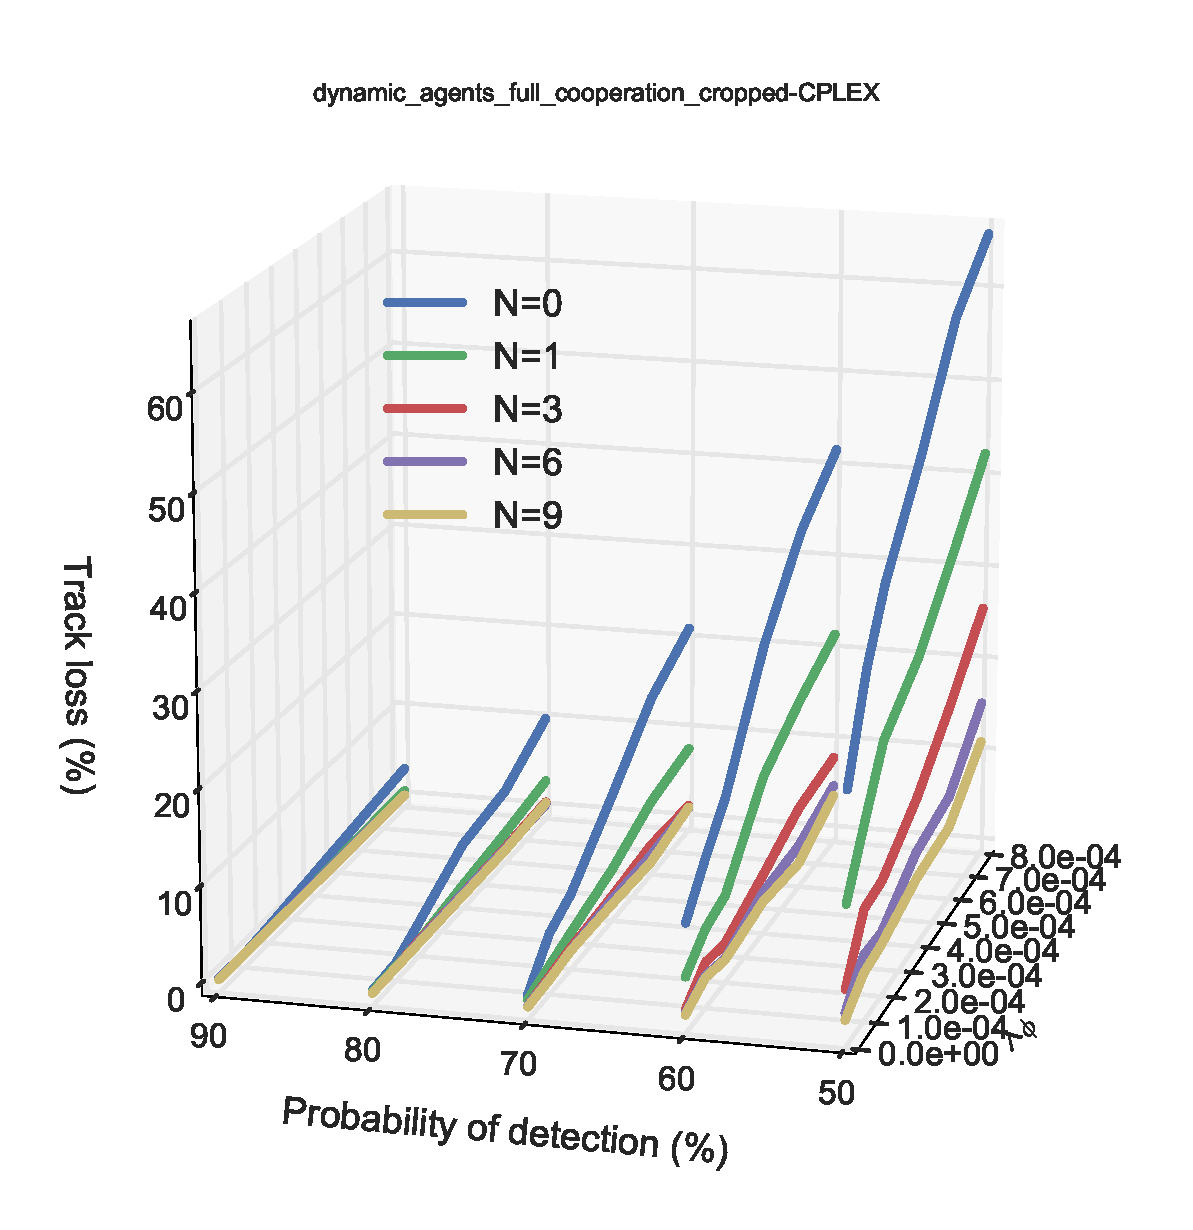
\includegraphics[clip,  trim=0cm 0cm 0cm 2cm,width=\textwidth]{dynamic_agents_full_cooperation_cropped-CPLEX}
        \caption{CPLEX solver}
    \end{subfigure}
    \begin{subfigure}{0.49\textwidth}
        \centering
        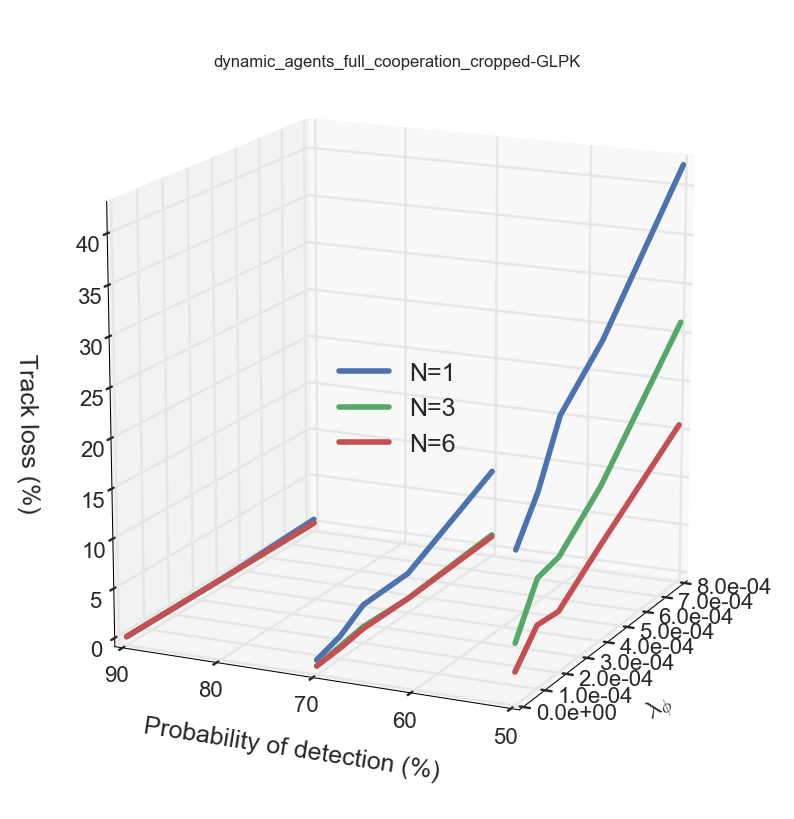
\includegraphics[clip,  trim=0cm 0cm 0cm 2cm,width=\textwidth]{dynamic_agents_full_cooperation_cropped-GLPK}
        \caption{GLPK solver}
    \end{subfigure}
    \begin{subfigure}{0.49\textwidth}
        \centering
        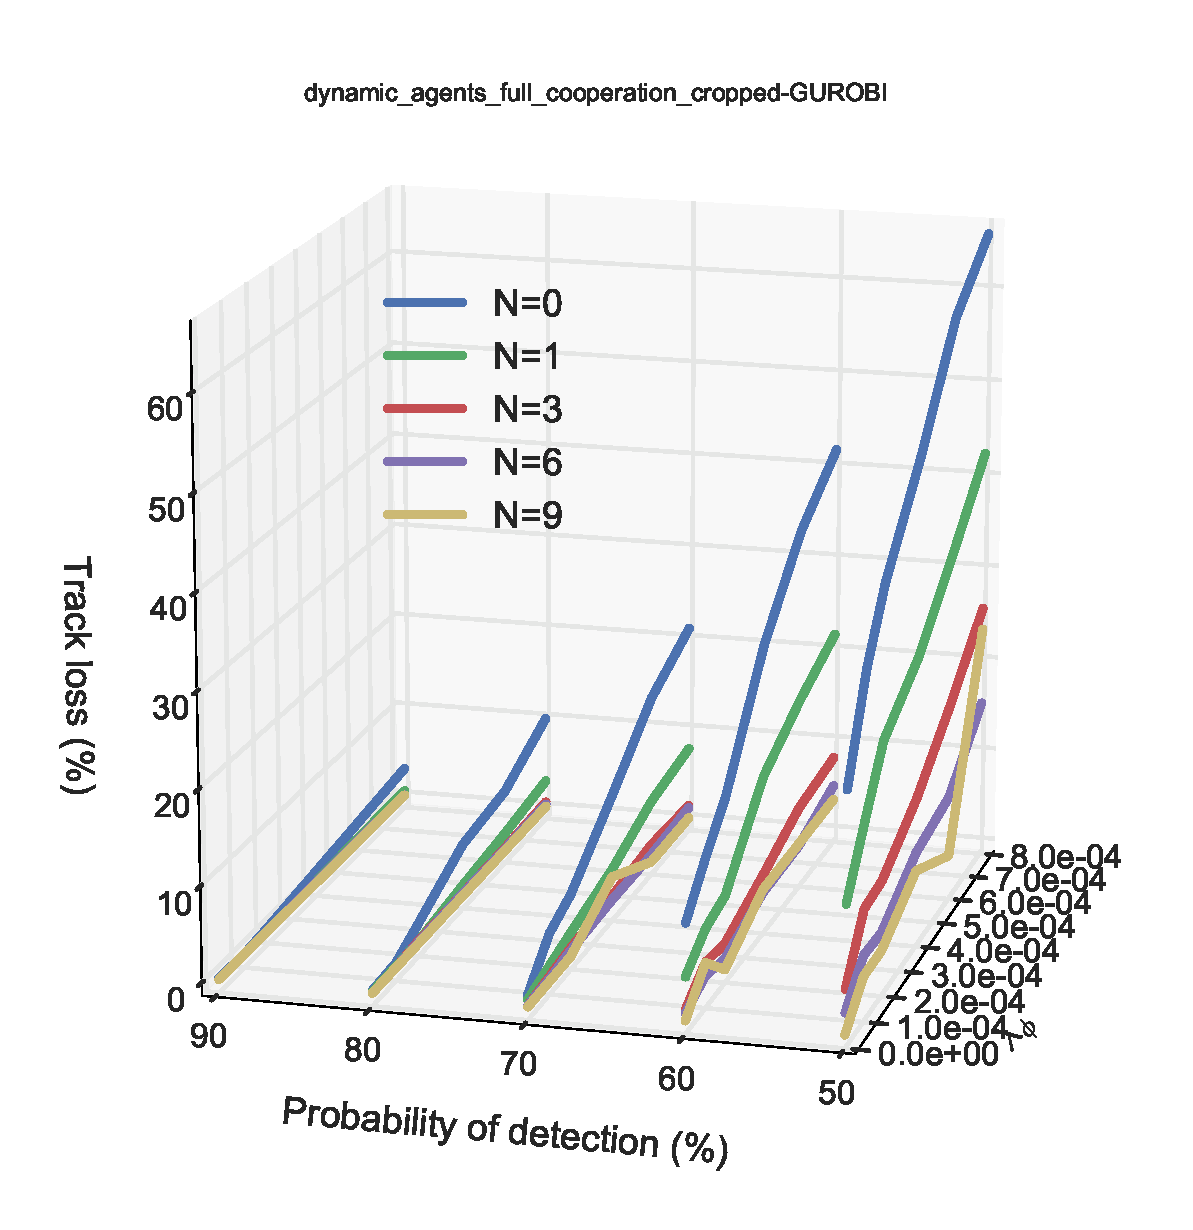
\includegraphics[clip,  trim=0cm 0cm 0cm 2cm,width=\textwidth]{dynamic_agents_full_cooperation_cropped-GUROBI}
        \caption{GUROBI solver}
    \end{subfigure}
	\label{fig:dynamic_agents_full_cooperation_cropped}
	\caption{Simulation results for all solvers in scenario 1}
\end{figure}

\begin{figure}[H]
    \centering
    \textbf{Scenario 2}\par \medskip
    \begin{subfigure}{0.49\textwidth}
        \centering
        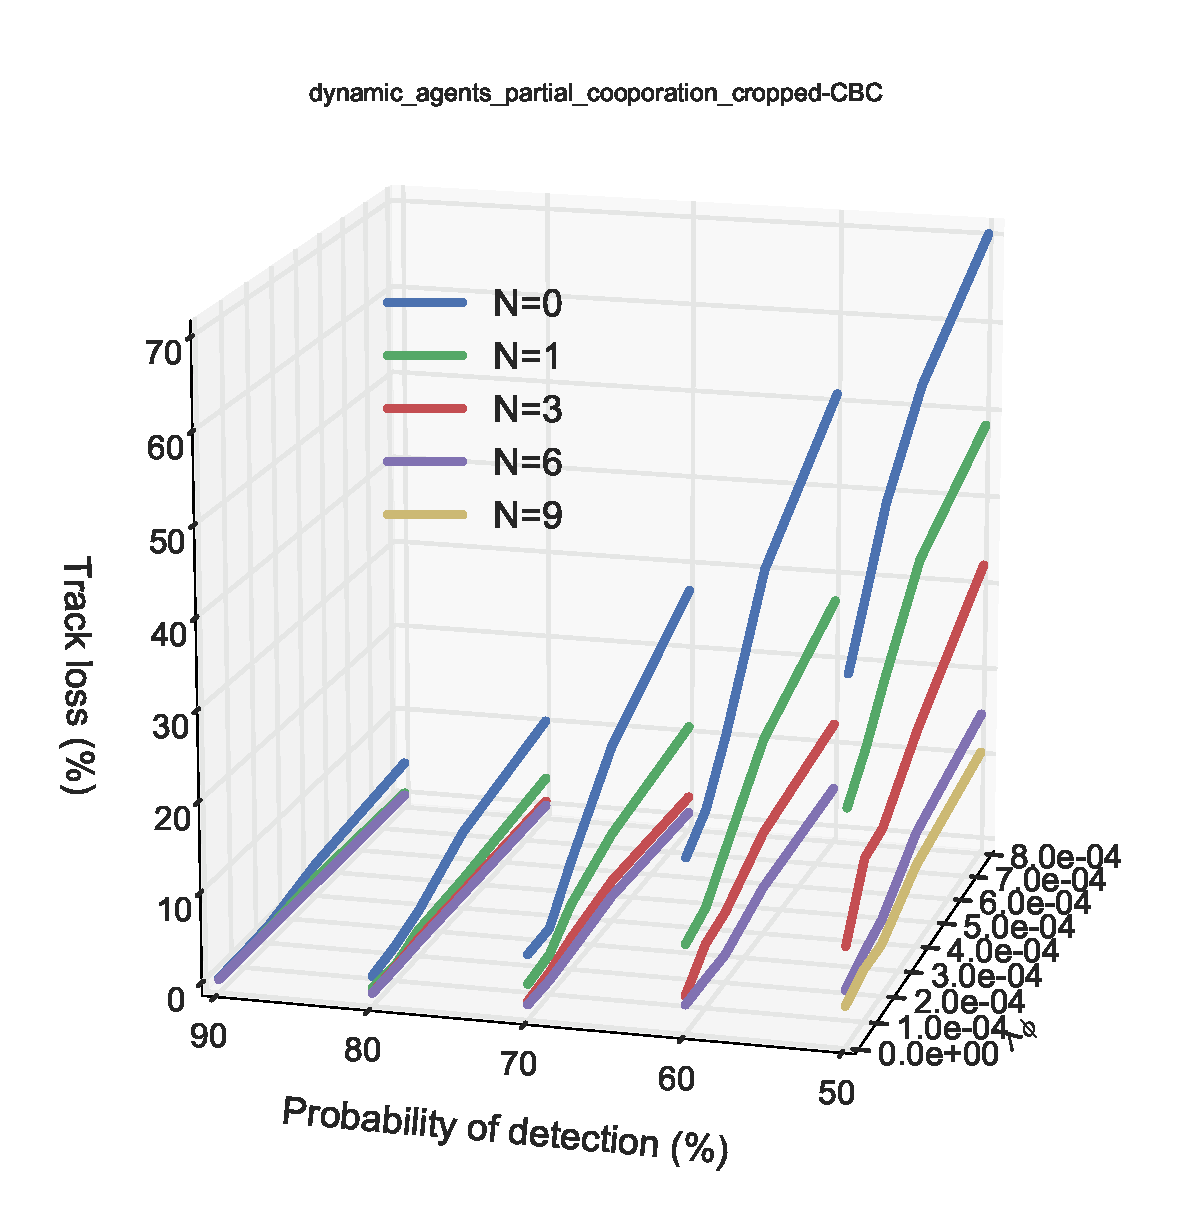
\includegraphics[clip,  trim=0cm 0cm 0cm 2cm, width=\textwidth]{dynamic_agents_partial_cooporation_cropped-CBC}
        \caption{CBC solver}
    \end{subfigure}
    \begin{subfigure}{0.49\textwidth}
        \centering
        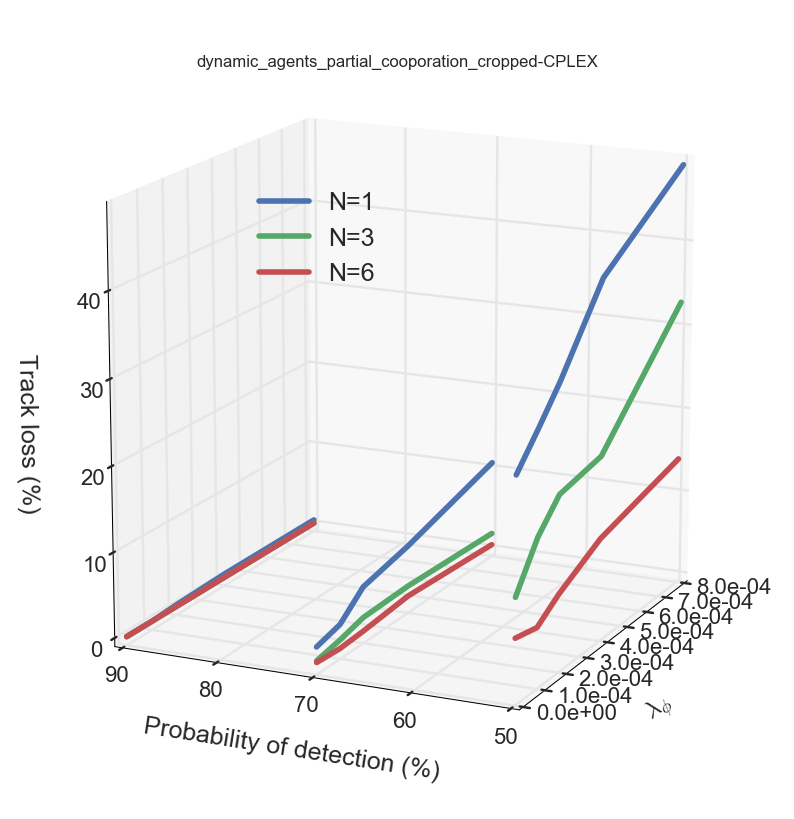
\includegraphics[clip,  trim=0cm 0cm 0cm 2cm,width=\textwidth]{dynamic_agents_partial_cooporation_cropped-CPLEX}
        \caption{CPLEX solver}
    \end{subfigure}
    \begin{subfigure}{0.49\textwidth}
        \centering
        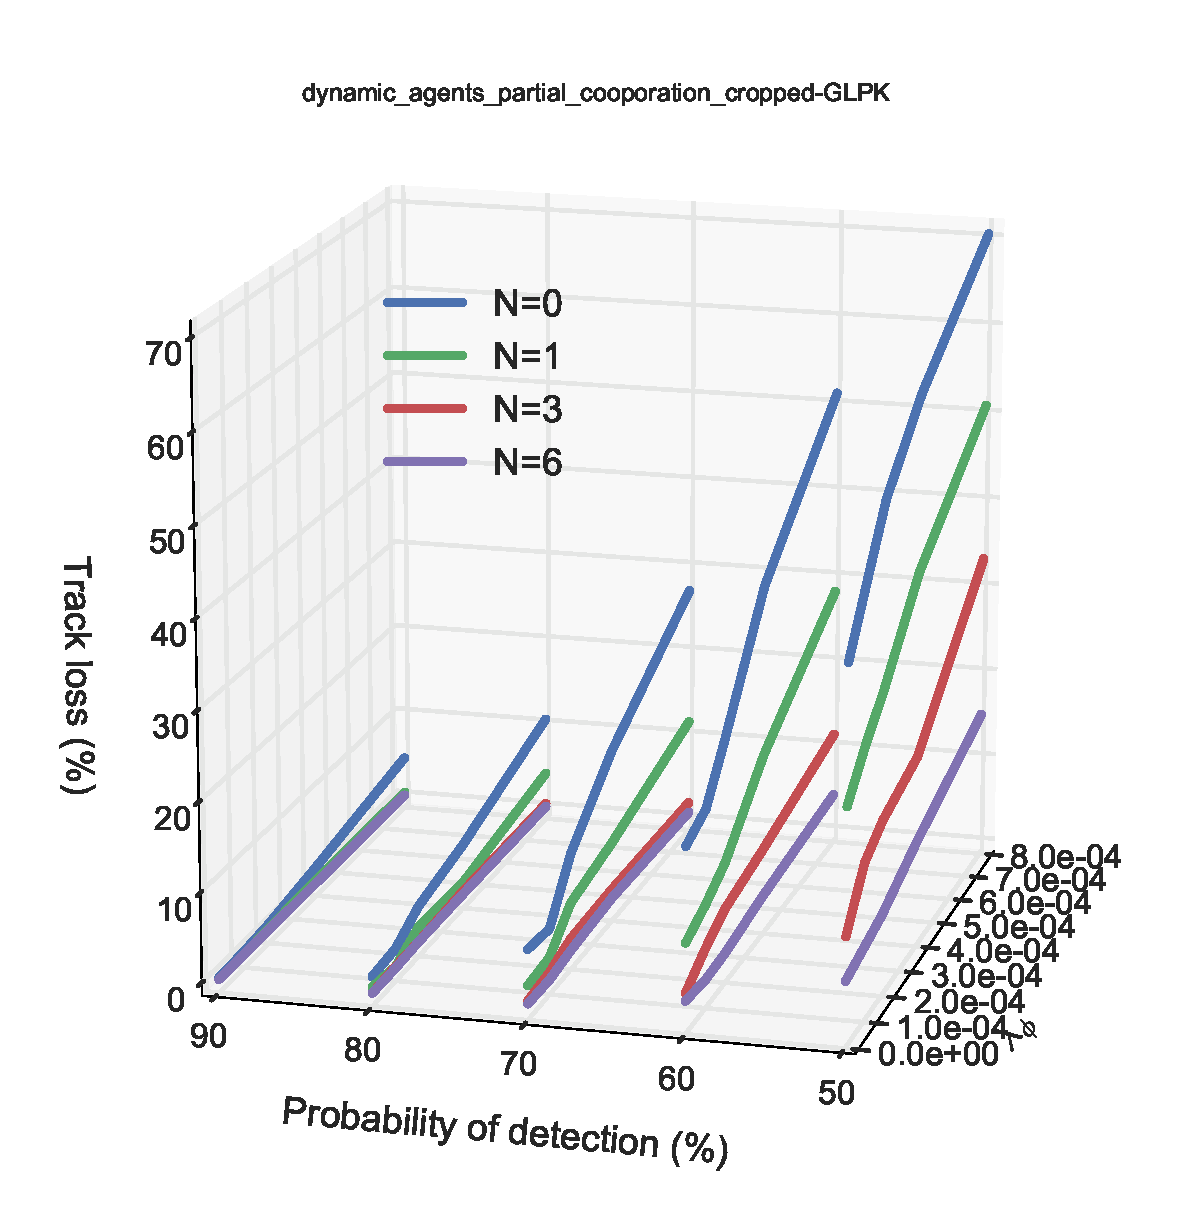
\includegraphics[clip,  trim=0cm 0cm 0cm 2cm,width=\textwidth]{dynamic_agents_partial_cooporation_cropped-GLPK}
        \caption{GLPK solver}
    \end{subfigure}
    \begin{subfigure}{0.49\textwidth}
        \centering
        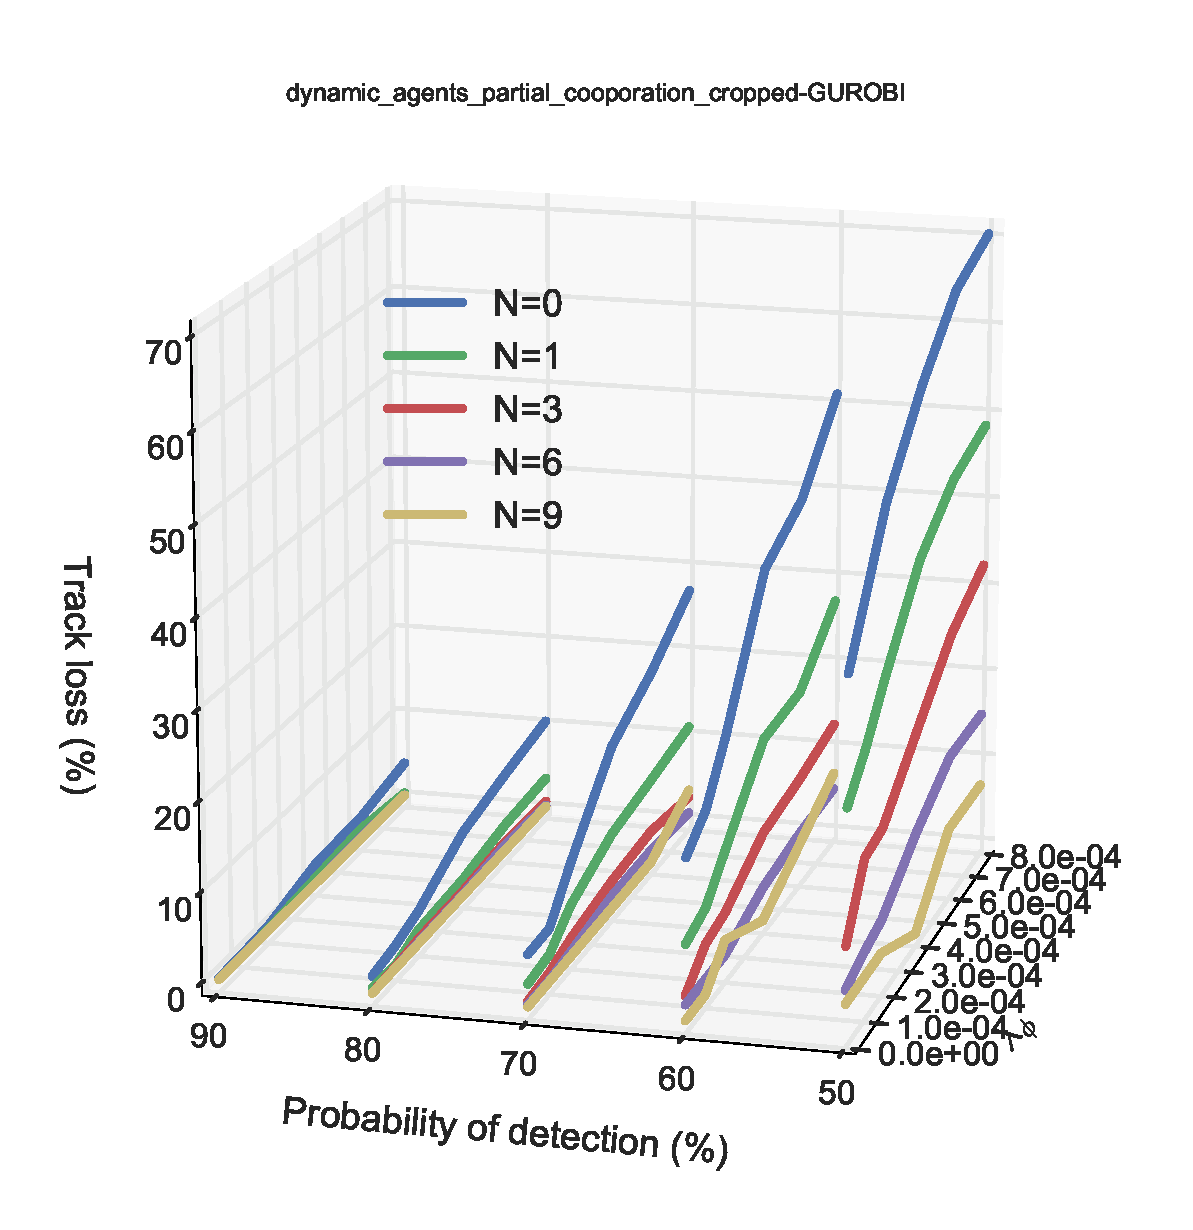
\includegraphics[clip, trim=0cm 0cm  0cm 2cm,width=\textwidth]{dynamic_agents_partial_cooporation_cropped-GUROBI}
        \caption{GUROBI solver}
    \end{subfigure}
	\label{fig:dynamic_agents_partial_cooperation_cropped}
	\caption{Simulation results for all solvers in scenario 2}
\end{figure}

\begin{figure}[H]
    \centering
    \textbf{Scenario3}\par \medskip
    \begin{subfigure}{0.49\textwidth}
        \centering
        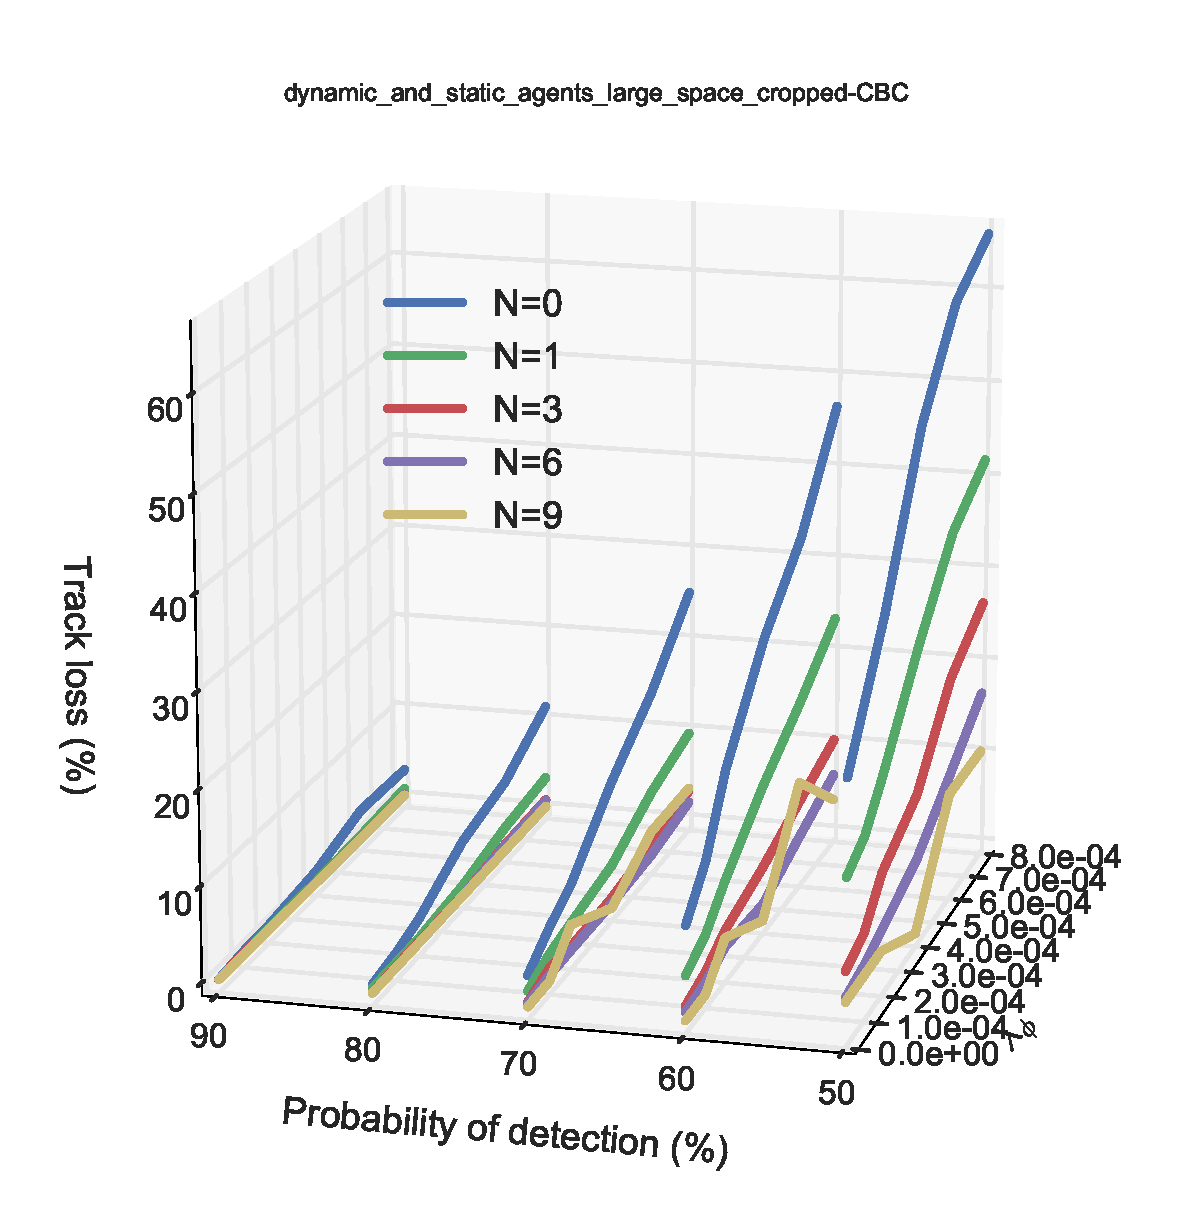
\includegraphics[clip, trim=0cm 0cm 0cm 2cm, width=\textwidth]{dynamic_and_static_agents_large_space_cropped-CBC}
        \caption{CBC solver}
    \end{subfigure}
    \begin{subfigure}{0.49\textwidth}
        \centering
        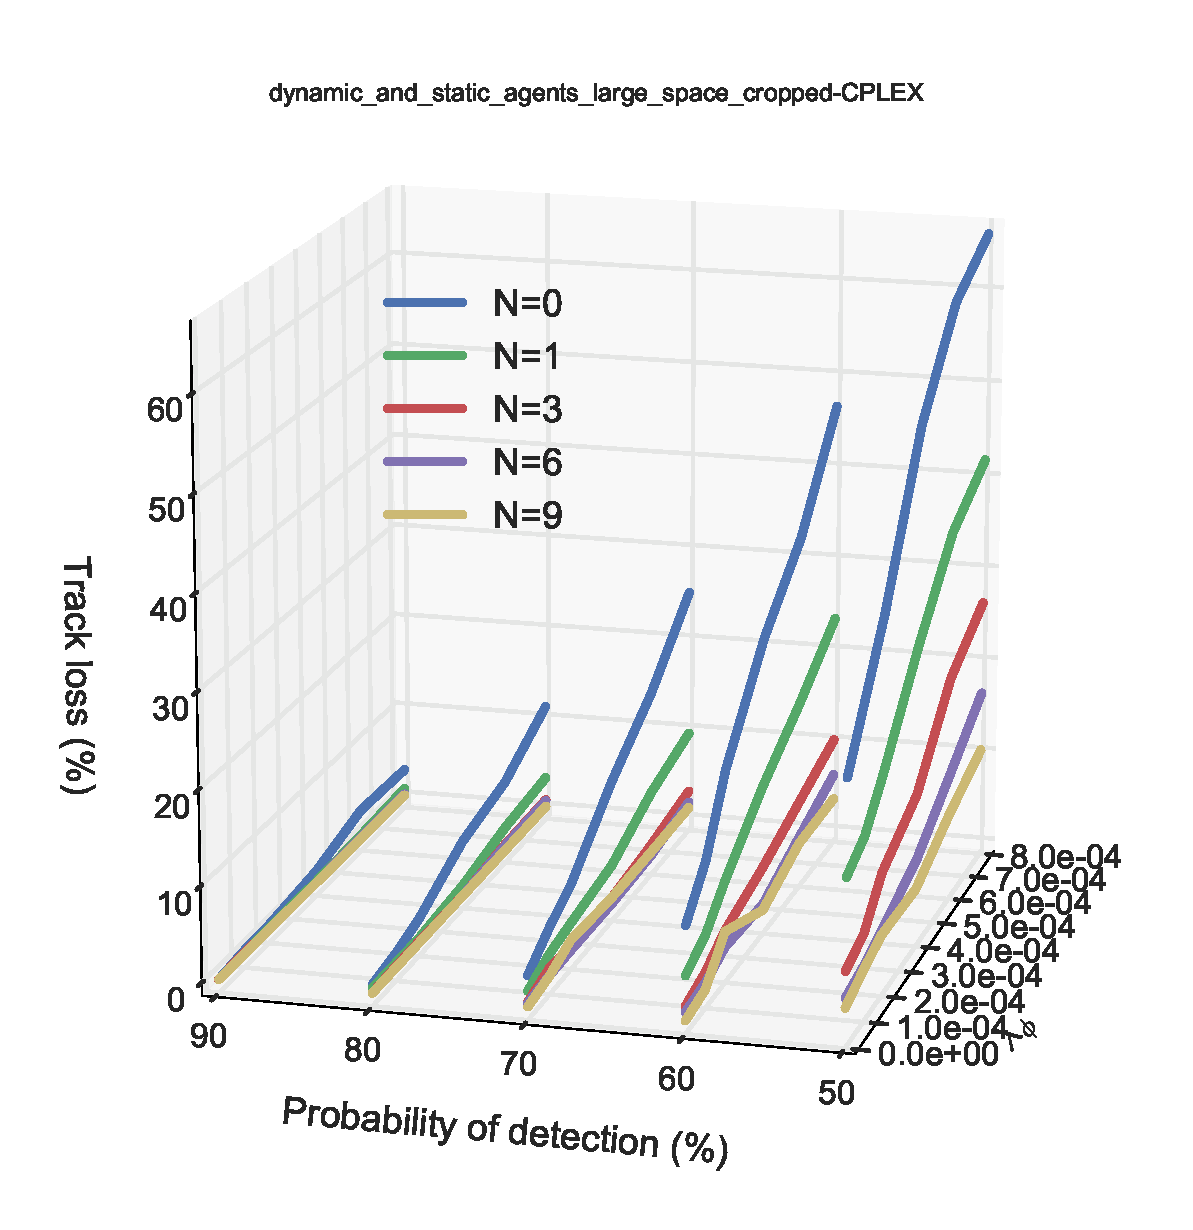
\includegraphics[clip, trim=0cm 0cm 0cm 2cm,width=\textwidth]{dynamic_and_static_agents_large_space_cropped-CPLEX}
        \caption{CPLEX solver}
    \end{subfigure}
    \begin{subfigure}{0.49\textwidth}
        \centering
        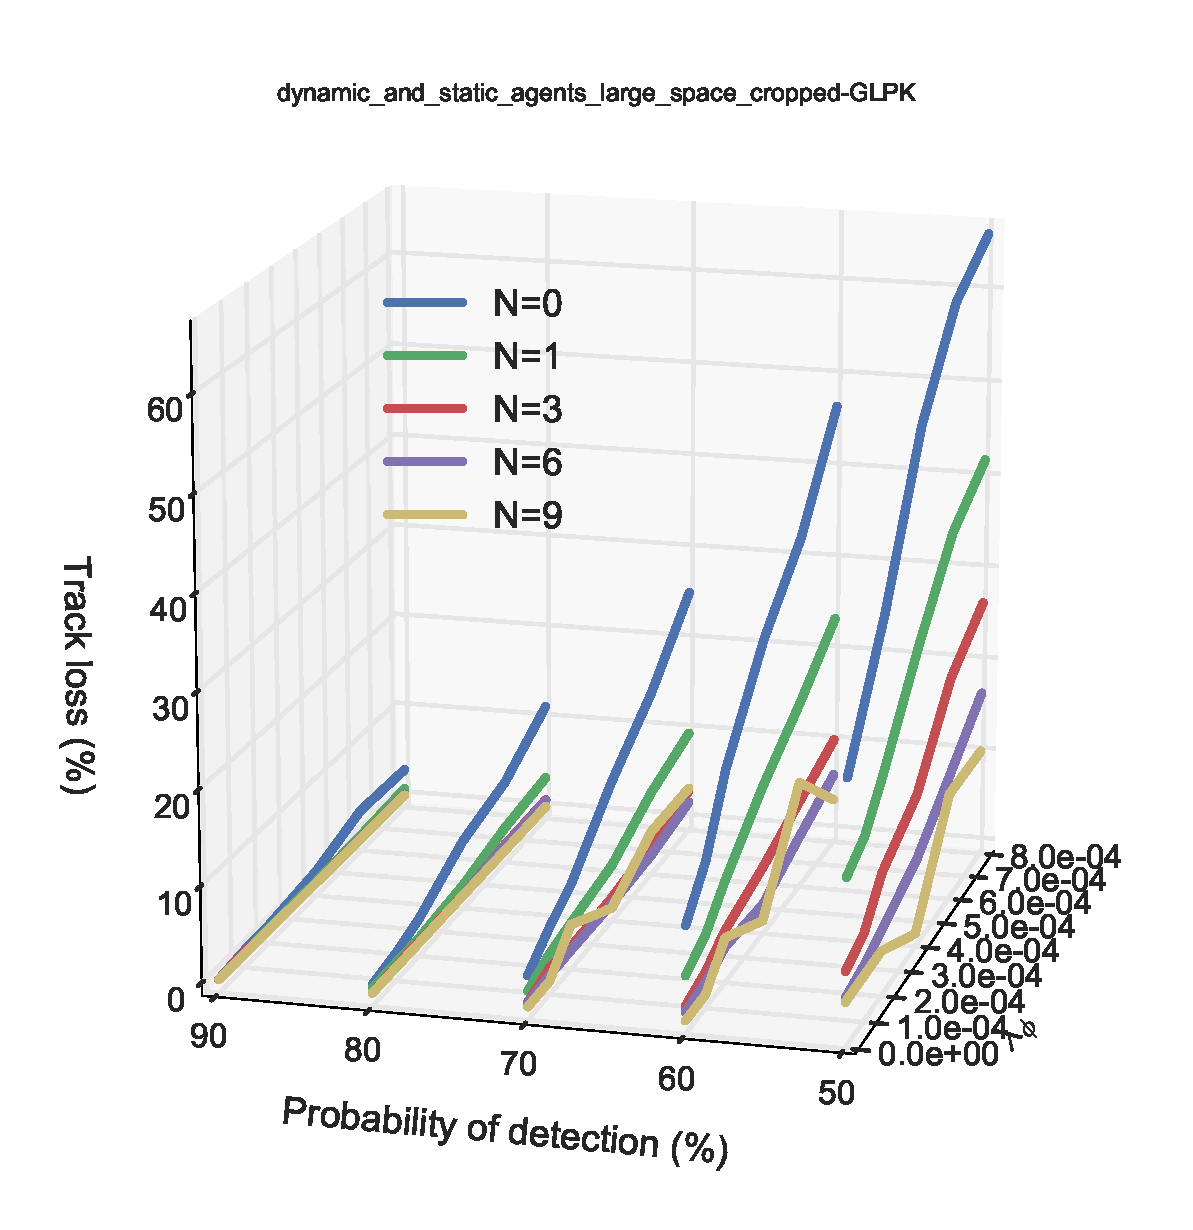
\includegraphics[clip, trim=0cm 0cm 0cm 2cm,width=\textwidth]{dynamic_and_static_agents_large_space_cropped-GLPK}
        \caption{GLPK solver}
    \end{subfigure}
    \begin{subfigure}{0.49\textwidth}
        \centering
        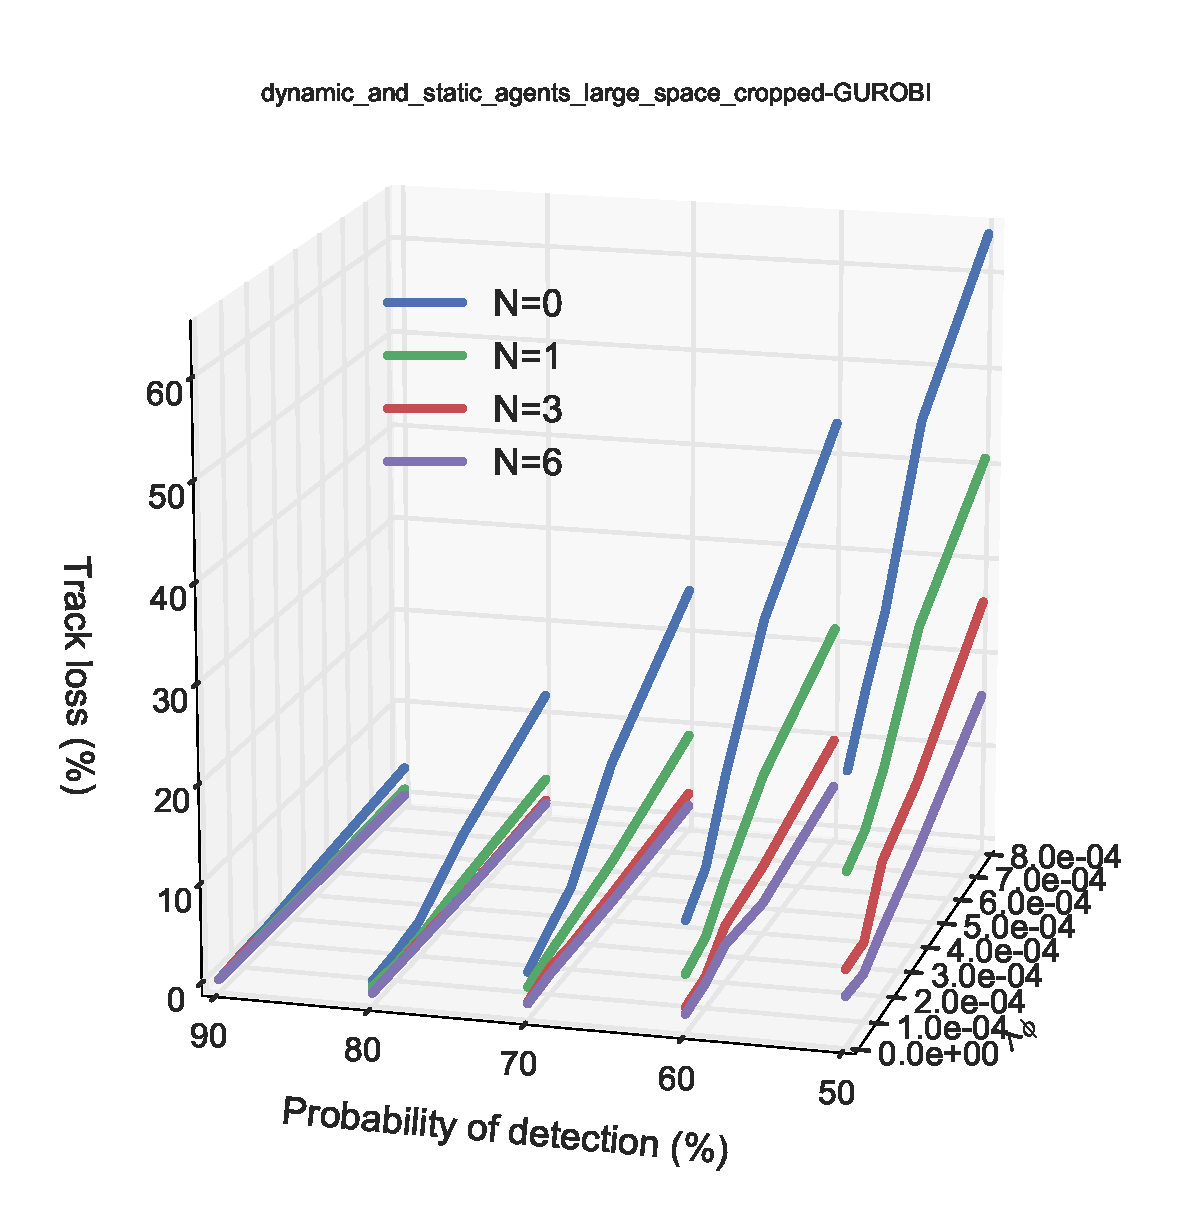
\includegraphics[clip, trim=0cm 0cm 0cm 2cm,width=\textwidth]{dynamic_and_static_agents_large_space_cropped-GUROBI}
        \caption{GUROBI solver}
    \end{subfigure}
	\label{fig:dynamic_and_static_agents_large_space_cropped}
	\caption{Simulation results for all solvers in scenario 3}
\end{figure}

\begin{figure}[H]
    \centering
    \textbf{Scenario 4}\par \medskip
    \begin{subfigure}{0.49\textwidth}
        \centering
        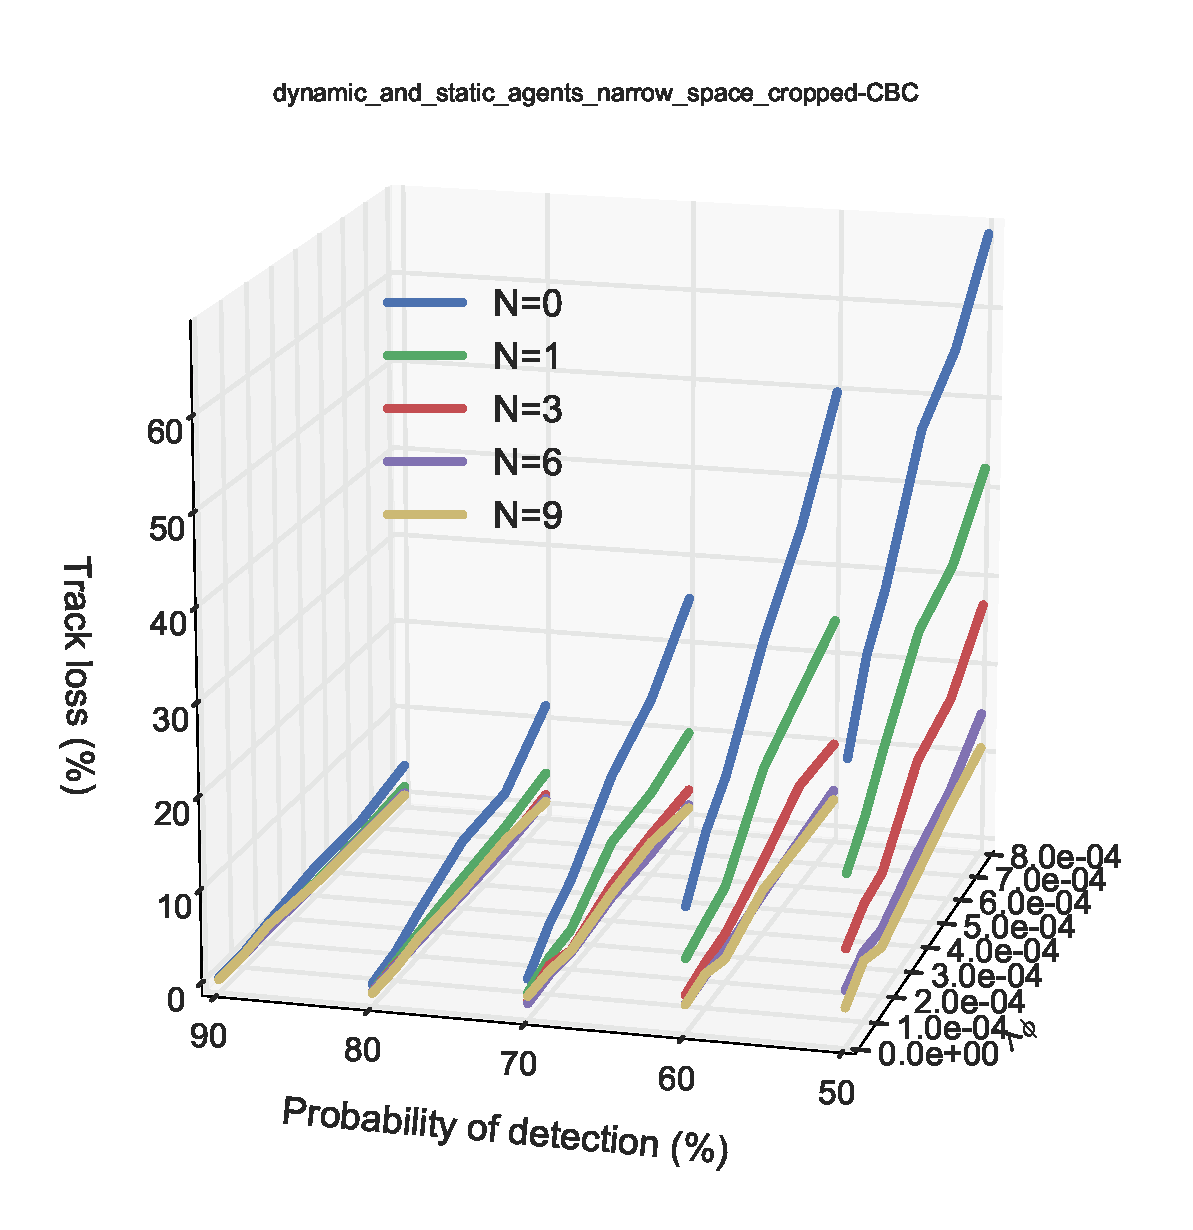
\includegraphics[clip,  trim=0cm 0cm 0cm 2cm, width=\textwidth]{dynamic_and_static_agents_narrow_space_cropped-CBC}
        \caption{CBC solver}
    \end{subfigure}
    \begin{subfigure}{0.49\textwidth}
        \centering
        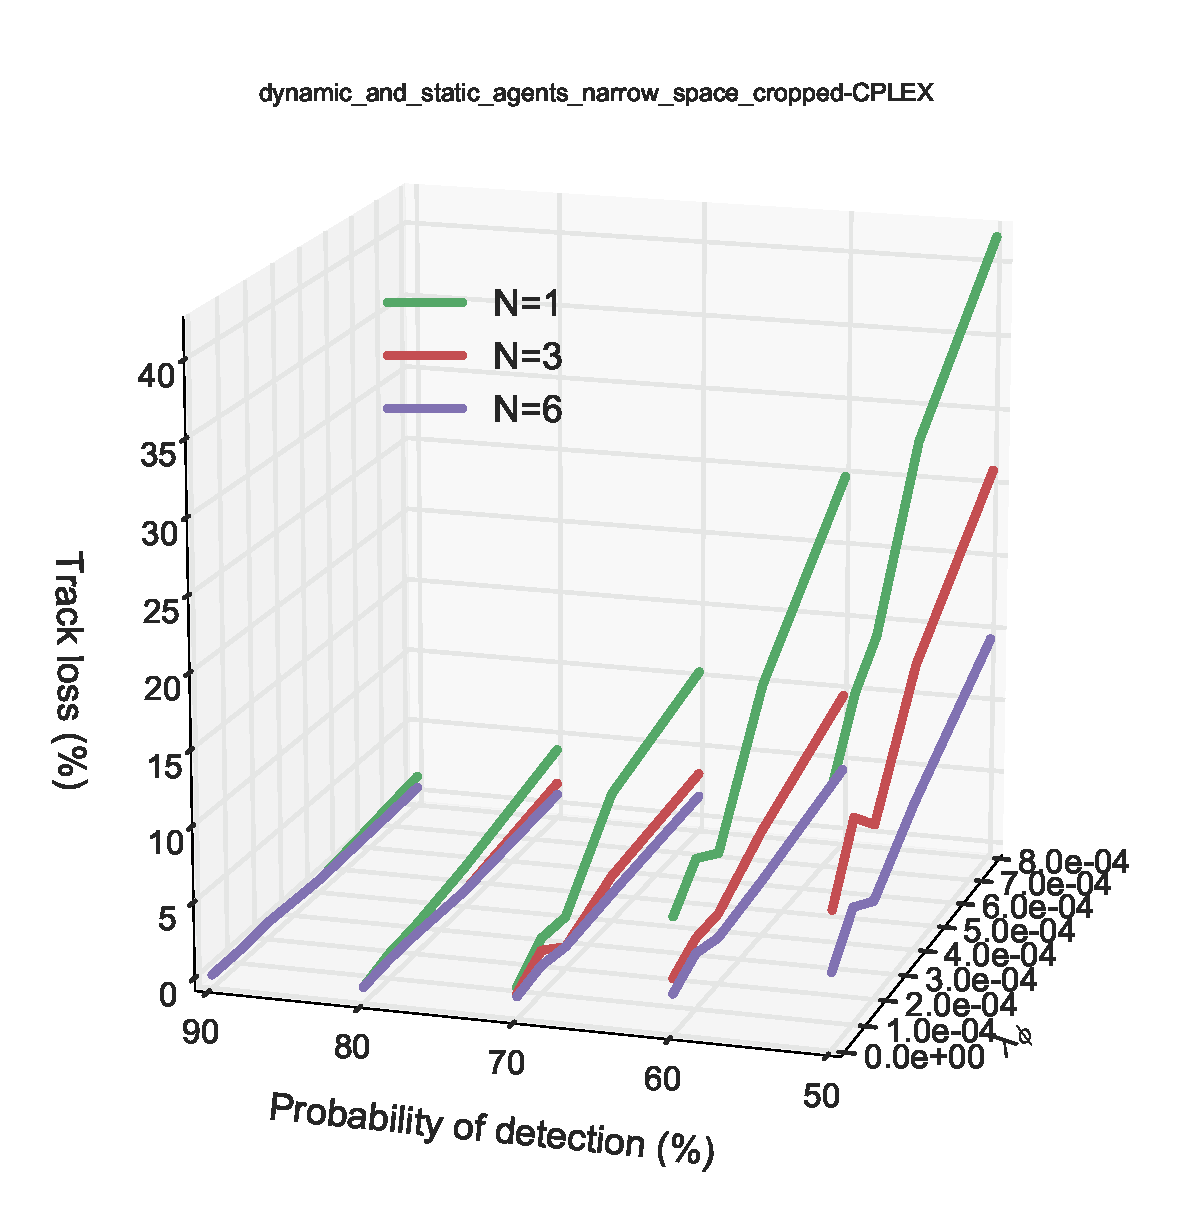
\includegraphics[clip, trim=0cm 0cm 0cm 2cm,width=\textwidth]{dynamic_and_static_agents_narrow_space_cropped-CPLEX}
        \caption{CPLEX solver}
    \end{subfigure}
    \begin{subfigure}{0.49\textwidth}
        \centering
        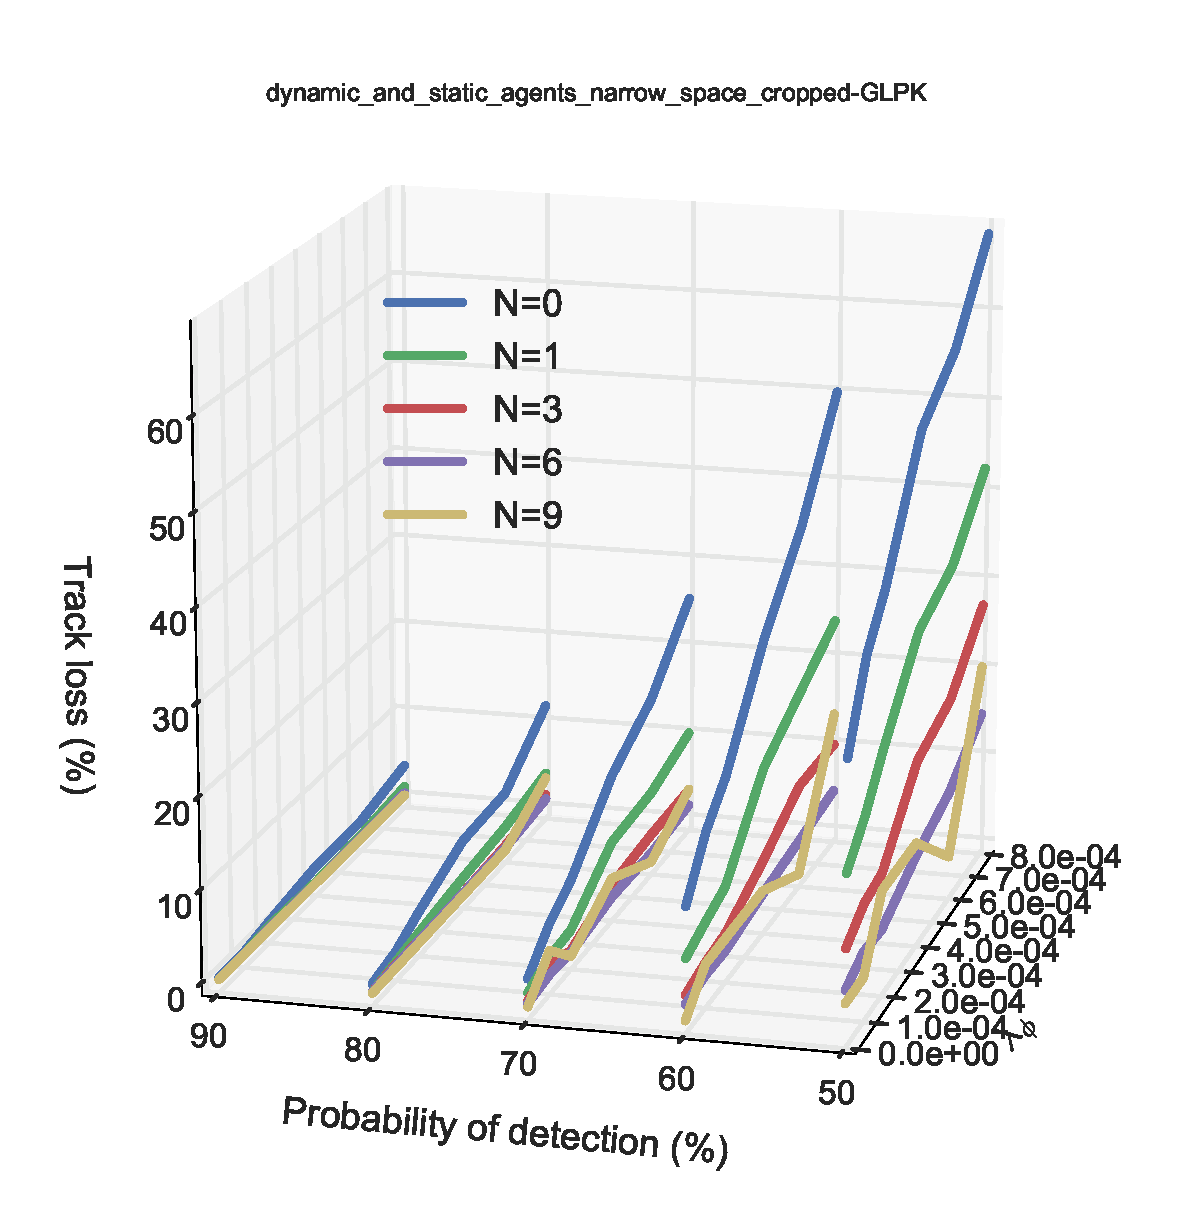
\includegraphics[clip, trim=0cm 0cm 0cm 2cm,width=\textwidth]{dynamic_and_static_agents_narrow_space_cropped-GLPK}
        \caption{GLPK solver}
    \end{subfigure}
    \begin{subfigure}{0.49\textwidth}
        \centering
        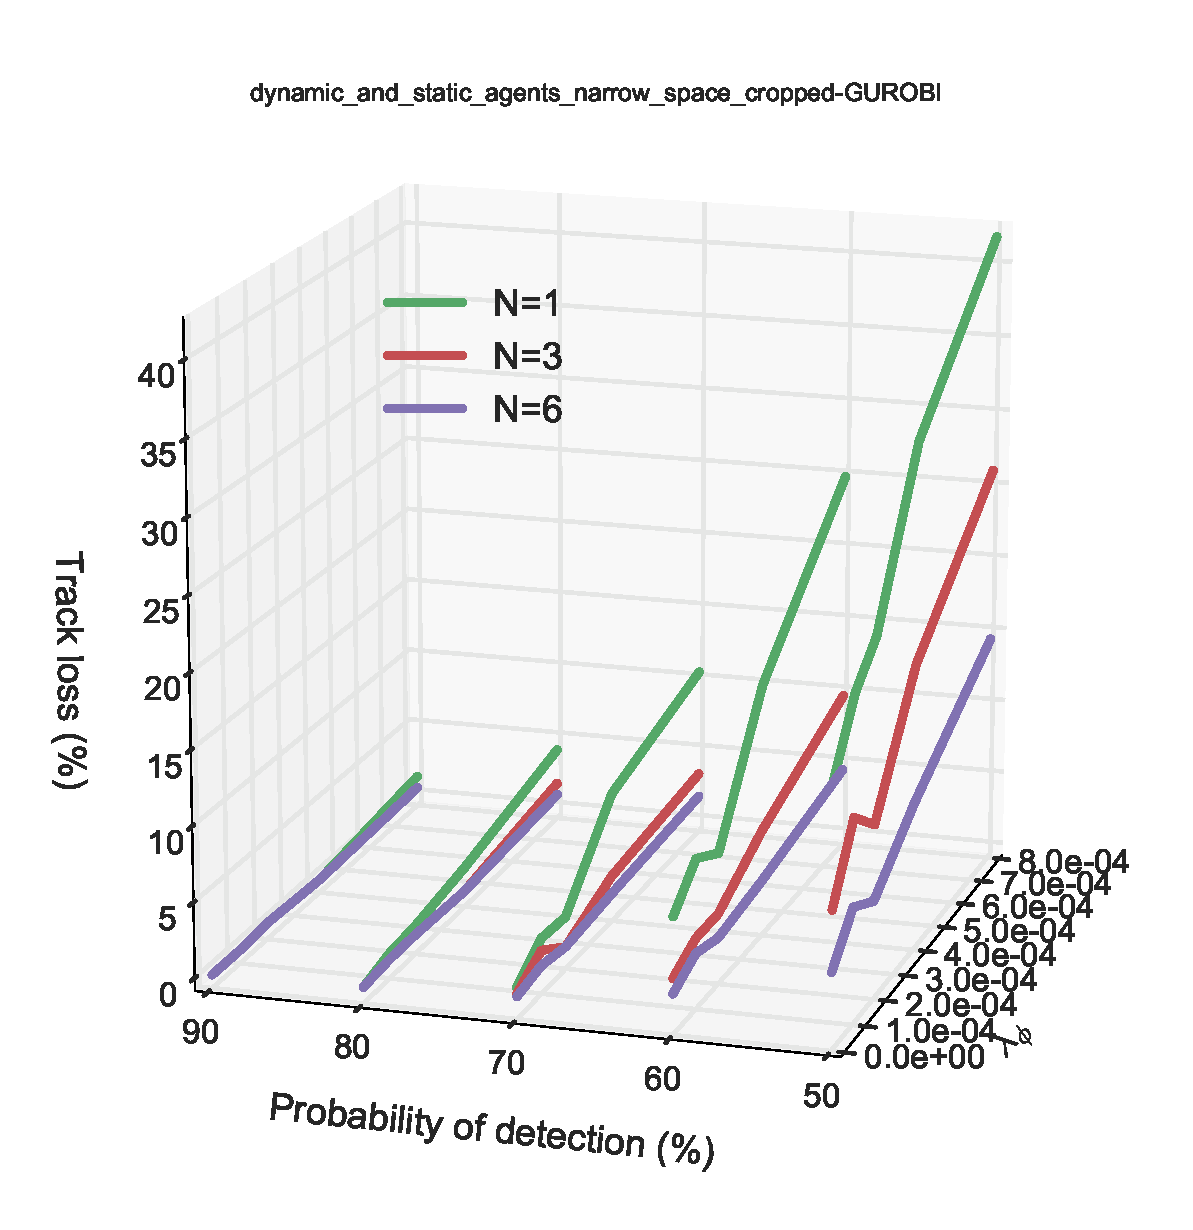
\includegraphics[clip, trim=0cm 0cm 0cm 2cm,width=\textwidth]{dynamic_and_static_agents_narrow_space_cropped-GUROBI}
        \caption{GUROBI solver}
    \end{subfigure}
	\label{fig:dynamic_and_static_agents_narrow_space_cropped}
	\caption{Simulation results for all solvers in scenario 4}
\end{figure}


\subsection{Runtime}
\subsubsection{Solvers}

\begin{tabular}{ r c c c c c c}
nHyp 	& CPLEX & GLPK 	& CBC	& SYMPHONY	& Gurobi	& Xpress	\\ \hline
13 		& 0.111	& 6 	& 6		& 6			& 6			& 6			\\
34 		& 0.106	& 9		& 9		& 6			& 6			& 6			\\
78 		& 0.106	& 9		& 9		& 6			& 6			& 6			\\
87 		& 0.108	& 9		& 9		& 6			& 6			& 6			\\
162 	& 0.112	& 9		& 9		& 6			& 6			& 6			\\
189 	& 0.115	& 9		& 9		& 6			& 6			& 6			\\
423 	& 0.130	& 9		& 9		& 6			& 6			& 6			\\
\end{tabular}